\section[The 1D Tight Binding Model for Electrons]{\hyperlink{toc}{The 1D Tight Binding Model for Electrons}}


 \begin{itemize}
     \item "Hopping of an electron along a 1D lattice.
     \item each atom has 1 orbital denoted by $\ket{n}$
     \begin{itemize}
         \item orthogonal to eachother $\Braket{n|m} = \delta_{n,m}$ although the true Kronecker-Delta function result is only really true if the atoms are far enough away from each other.
     \end{itemize}
     \item Wave function of the electron in the basis of the orbitals is:
     \[\ket{\Psi} = \sum_n c_n \ket{n} \]
     \item Model of linear combination of atomic orbitals (LCAO) 
     \item Time Independent Schrodinger Equation (TISE):
     \[ H \ket{\Psi} = E \ket{Psi}\]
     \item Hamiltonian only couples nearest neighbour sites so we say:
     \[ \braket{n | H | m} = \begin{cases}
     \epsilon_0, \qquad n=m \leftarrow \text{staying in atom} \\
     -J, \qquad n=m\pm1  \leftarrow \text{ hop by 1 site is way more probable} \\
     0, \qquad \text{otherwise} \leftarrow \text{than hopping by severeal atoms.}
     \end{cases}\]
     
     \[ \braket{n | H | m} = \begin{bmatrix} 
    \epsilon & -J & &\text{\huge0} &\\
    -J & \epsilon & -J & & \\
    & -J & \ddots & \ddots & \\
    \text{\huge0} & & \ddots & &
    \end{bmatrix}
    \]
    \[ \braket{n|\mathcal{H}|m} = \epsilon_0 \delta_{n,m} - J(\delta_{n,m+1} + \delta_{n, m-1})\]
    \[ \sum_m H_{n,m} c_m = E c_n \]
    TISE: \[ \epsilon_0 c_n - J (c_{n-1} + c_{n+1}) = E c_n\]
    Plug-in Ansatz (without time dependancy): \[ c_n = \frac{e^{-ikna}}{\sqrt{N}} \] 
    Relationship to phonons -- obtain disperesion relation:
    \[ E = \epsilon_0 - 2J \cos(ka) \]
    We get single band because we chose to have 1 orbital per site with our current model.
    \item \textbf{Phonons} in \textbf{monatomic chain} $\rightarrow$  \textbf{ diatomic or more complex crystals} \\
    \vspace{7px}
    similar to 
    \item \textbf{Band Diagram} in \textbf{1 orbital per site} $\rightarrow$ \textbf{multiple orbitals per site}
    \item We can represent \textbf{band structure} (energy ranges and k-dependence of multiple bands.
    \item Reduced zone scheme vs Extended zone scheme
    \begin{figure}
        \centering
        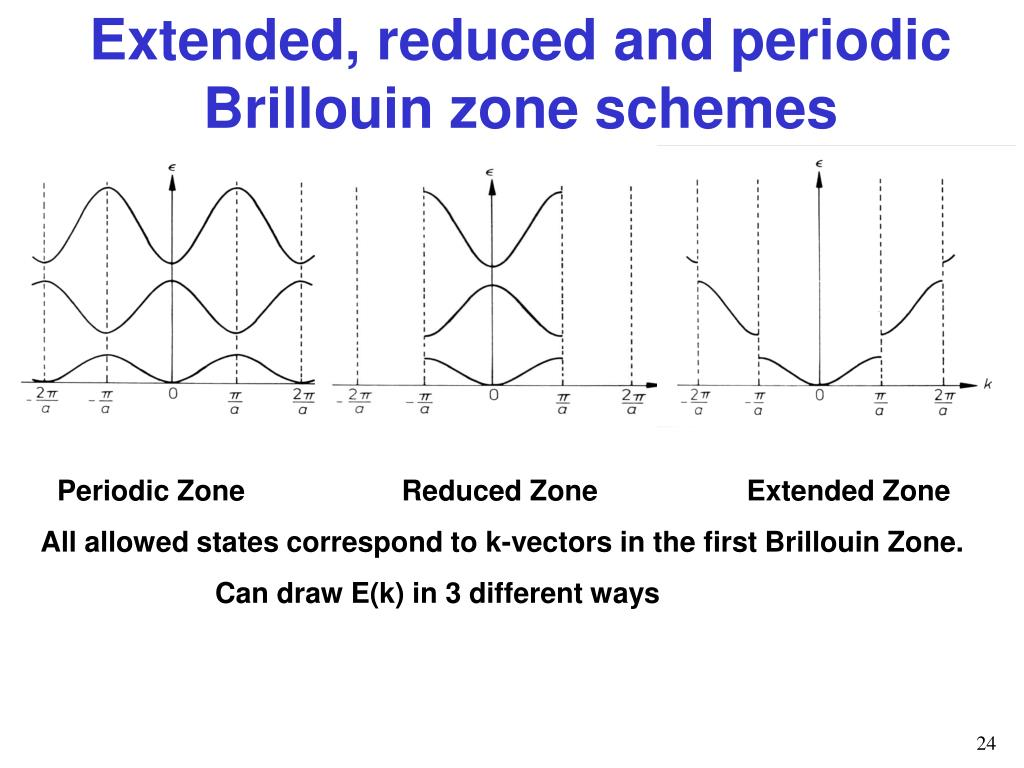
\includegraphics[width = 0.75 \linewidth]{Images/extended-reduced-and-periodic-brillouin-zone-schemes-l.jpg}
        \caption{Caption}
        \label{fig:brillouin zone}
    \end{figure}
    \item Typically many bands in solids with 2 relevant bands
    \item no solutions for any energy in this gap which relates to insulators, conductors, semiconductors etc.
    \item energy gap = band gap, and occurs at edge of Brillouin zone for the extended zone scheme.
    \item \textbf{Bandwidth} effective mass and crystal momentum
    \item width of the band energy depends of nuclei spacing
    \item N lattice sites + one orbital $\rightarrow$ N states for electron.
    \item $\frac{2 \pi}{aN}$ spacing is so incredibly small for all particle solids so we therefore assume band structure is continuous.
    \item \textbf{Band Shape}\\
    Approximate for $k\ll 1$ we see parabolic near k=0 for free particle $E=\frac{p^2}{2m} = \frac{\hbar^2k^2}{2m}$.
    \[E = \epsilon_0 -2J \cos(ka)\]
    \[E \approx \epsilon_0 - 2J(1-\frac{(ka)^2}{2})\]
    \[E \approx \epsilon_0 -2J + Ja^2k^2 \]
    \[E = \frac{\hbar^2 k^2}{2m^*}+ \text{Const.}\]
    \[\frac{\hbar^2 k^2}{2m^*} = Ja^2 k^2 \]
    Effective Mass (determined by J: hopping parameter/ tunnelling amplitude):
    \[ m^* = \frac{\hbar^2}{2Ja^2} \]
    \textbf{Filling Bands and the Fermi Surface}
    \item atoms with one valence electron, expect donate to collection moving in band.
    \item electrons have 2 spin ($\uparrow$, $\downarrow$) which gives room for 2N electrons in band.
    \item at low temp ($ T \ll T_f$), half filled band involves states being filled up to the Fermi Energy.
    \item system has fermi surfaces (here only 2 points) k points where the filled meets unfilled region.
    \item c $\propto$ T: heat capacity propto temp
    \item \textbf{Metal}: the fermi surface is in the middle of a band.
    \item applied external electrical field, electrons can accelerate to higher values of k $\rightarrow$ current flows in material. (backward and forward moving).
    \item \textbf{Band Insulator}: if band is filled, fermi surface is at the edge of the Brillouin Zone, then there are no states available in band for electrons to move into by an electrical field. (almost never carries current)
    \item \textbf{Energy Gap} \\
    $\rightarrow$ if it's large enough it's snot possible for electron to be pushed to higher band.\\
    $\rightarrow$ if BG $\ge 4eV$ then material is an (band) insulator.\\
    $\rightarrow$ if BG $<$ 4eV then electrons can be transferred to higher bands either @ \textbf{finite temperatures} or with \textbf{applications of fields} $\rightarrow$ material can then be a semiconductor.
    \item Many materials with \textbf{2 valence electrons} are insulators $\rightarrow$ some can form metals if interatomic spacing is small enough (two bands merge). See E bands vs atomic spacing.
    \item \textbf{Opposite} many materials with 1 valence electron are metals $\rightarrow$ some are special type of Insulator: "Mott Insulator"
    \item too much energy to have 2 electrons (ex. NiO $\&$ CoO) on one site.
    \item Simple band model also doesn't fully describe when system has magnetic properties (ferro, antiferro, $\&$ ferro) spin alignment.
    \item kwant simulation library in PYTHON is a cool resource.
 \end{itemize}
